%% Two-column ICML 2026 style, preprint option, anonymous authors.
\documentclass{article}

\usepackage[T1]{fontenc}
\usepackage{microtype}
\usepackage{graphicx}
\usepackage{booktabs}
\usepackage{multirow}
\usepackage{array}
\usepackage{xurl}
\usepackage{hyperref}
\newcommand{\theHalgorithm}{\arabic{algorithm}}

\usepackage[preprint]{icml2026}

\usepackage{amsmath}
\usepackage{amssymb}
\usepackage{tikz}
\usetikzlibrary{positioning,arrows.meta}
\usepackage[capitalize,noabbrev]{cleveref}

\newcommand{\pend}{\textit{pending}}
\newcommand{\na}{--}
\newcolumntype{L}[1]{>{\raggedright\arraybackslash}p{#1}}

\icmltitlerunning{A Single-Pass Decision Model as a Mobile Agent}

\begin{document}

\twocolumn[
  \icmltitle{A 2B Single-Pass Decision Model as a Mobile Agent:\\
    Per-Step Accuracy, Task Success, and What the Gap Is Made Of}

  \icmlsetsymbol{equal}{*}

  \begin{icmlauthorlist}
    \icmlauthor{Anonymous Author(s)}{anon}
  \end{icmlauthorlist}

  \icmlaffiliation{anon}{Anonymous institution}
  \icmlcorrespondingauthor{Anonymous Author(s)}{anonymous@example.com}

  \icmlkeywords{GUI agents, decision models, AndroidWorld, AndroidControl, evaluation}

  \vskip 0.3in
]

\printAffiliationsAndNotice{}

\begin{abstract}
We turn a 2B \emph{decision model}, LiquidAI's d1-2B, into a mobile agent.
At every step the model reads the screenshot, the goal, its own action history and the
screen's accessibility elements once. It then answers a fixed set of typed questions in a
single forward pass and generates no tokens. The questions are: which action, which
element, which scroll direction, which app, and which span of the input to type or report.
We fine-tune on AndroidControl with synthetic augmentation. We add 1{,}736 goal-to-app rows
built from AndroidWorld's task generator; they cover 97 of the 116 evaluated templates. No
AndroidWorld rollout is used.

\textbf{Results.} On AndroidControl-High the model gets 61.7\% of steps right (5{,}213/8{,}444),
but only 22.3\% of episodes have every step right (344/1{,}543). On AndroidControl-Low the
figures are 89.3\% of steps and 60.4\% of episodes. Under the official AndroidWorld protocol
(116 tasks, seed 30, one attempt) it scores 25/115 = 21.7\%, at a median of 135\,ms per
decision.

\textbf{Analysis.} The episode-level AndroidControl rate and the AndroidWorld rate are nearly
equal, while the per-step rate suggests much more. We decompose the gap. Of the 91 failed
AndroidWorld tasks, 51 ended with a wrong ``done'' and 40 ran out of steps. About 36 need
abilities a single pass under our constraints does not have: arithmetic, dates, memory across
screens, and text that exists only in pixels. Harness and environment fixes alone moved the
score from 15.5 to 25 on a fixed checkpoint. We report negative results with the positive ones.
\end{abstract}

%% ------------------------------------------------------------------
\section{Introduction}

Published mobile GUI agents are almost all \emph{generative}. A vision-language model writes
a thought and an action string at each step, often over several calls (planner, actor,
reflector). A \emph{decision model} works another way. It reads the state once and returns
probabilities over options that the caller supplies, and it writes no free text
\cite{typesafe2026,liquidd12026}. For an on-device agent this offers three things: low latency,
an output schema that cannot be broken, and a confidence for each answer. Whether such a model
can \emph{act}, and not only classify, is an open question.

We study that question with measurements, not with a leaderboard claim. Our contributions:
\begin{enumerate}
  \item A \textbf{decision contract} for phone control: a text-and-image state, typed
        questions, and outputs that copy spans from the input. One function renders it for
        training, evaluation and serving.
  \item Results on AndroidControl (Low and High) in the standard Type / Grounding / SR format,
        and on AndroidWorld under its official protocol, each with its denominator.
  \item A breakdown of the gap between per-step accuracy and task success, based on a
        trace-level reading of all 91 failed AndroidWorld tasks.
  \item A record of what did not work, and of harness and environment defects that changed
        scores without any change to the model.
\end{enumerate}

%% ------------------------------------------------------------------
\section{Related Work}

\textbf{Generative mobile agents.} M3A, the reference agent of AndroidWorld, keeps a
per-step LLM summary as memory and reports 30.6\% with GPT-4 Turbo \cite{androidworld2024}.
UI-TARS \cite{uitars2025}, MAI-UI \cite{maiui2025}, GUI-Owl and Mobile-Agent-v3
\cite{mobileagentv3}, and UI-Venus-1.5 \cite{uivenus15} are end-to-end VLMs that generate
text. MobileRL adds online reinforcement learning on generated AndroidWorld task variants
\cite{mobilerl2025}. V-Droid scores candidate actions with a verifier and trains on AndroidWorld
apps and tasks \cite{vdroid2025}. AndroidGen collects its trajectories in the AndroidWorld
emulator and grows a retrieval database during evaluation \cite{androidgen2025}.
\Cref{tab:aw-context} lists their AndroidWorld numbers. These numbers are context, not a
ranking: model size, calls per step, generated reasoning, extra components and
benchmark-derived training data all differ, and none of them was produced by our harness.

\textbf{Decision models.} TypeSafe's Jev and LiquidAI's d1 answer typed questions (choice,
yes/no, score, span, box) in one pass \cite{typesafe2026,liquidd12026}. TypeSafe's guidance
says such models should ``keep math in code, which includes counting and date comparison''
\cite{typesafelimits2026}. Our failure analysis reaches the same point from the agent side
(\cref{sec:failures}).

\textbf{Data and per-step benchmarks.} AndroidControl gives a goal (High) and a per-step
instruction (Low) for 15{,}283 demonstrations \cite{androidcontrol2024}. Its usual scorer
compares each predicted step with the demonstrator's step, given the demonstrator's history.
AndroidControl-Curated cleans the test set and reports a per-step success rate
\cite{androidcontrolcurated2025}. AMEX adds element-level annotations and also reports only
per-step metrics \cite{amex2024}. None of these checks whether a task was completed.

\begin{table*}[t]
\centering
\caption{Published AndroidWorld success rates, for context only (not a ranking). Each value is
the paper's own report on the official task suite. ``--'' means we did not find the field in
the source. The AndroidGen percentages fit 111 tasks rather than 116 (our derivation).}
\label{tab:aw-context}
\footnotesize
\setlength{\tabcolsep}{3pt}
\begin{tabular}{@{}l l c c L{3.2cm} L{2.3cm} r@{}}
\toprule
Agent / model & Params & Calls & Text & AndroidWorld-derived training data & Extra components & SR (\%) \\
\midrule
\textbf{Ours: d1-2B} & 2B & 1 & no & goal-to-app rows from the task generator (97/116 templates) & none & \textbf{21.7} \\
M3A, GPT-4 Turbo \cite{androidworld2024} & -- & $\geq$2 & yes & no & step summary as memory & 30.6 \\
UI-TARS \cite{uitars2025} & -- & 1 & yes & not stated & -- & 46.6 \\
AndroidGen, GPT-4o \cite{androidgen2025} & -- & several & yes & trajectories collected in AndroidWorld & planner, retrieval, checks & 46.8 \\
MAI-UI-2B \cite{maiui2025} & 2B & 1 & yes & not stated & none & 49.1 \\
UI-Venus-1.5-2B \cite{uivenus15} & 2B & 1 & yes & not stated & -- & 55.6 \\
V-Droid \cite{vdroid2025} & 8B + LLM & several & yes & AndroidWorld apps and tasks & verifier & 59.5 \\
GUI-Owl-7B \cite{mobileagentv3} & 7B & 1 & yes & not stated & -- & 66.4 \\
Mobile-Agent-v3 \cite{mobileagentv3} & 32B & several & yes & not stated & manager, worker, reflector, notetaker & 73.3 \\
MAI-UI-235B-A22B \cite{maiui2025} & 235B & 1 & yes & not stated & none & 76.7 \\
MobileRL-9B \cite{mobilerl2025} & 9B & 1 & yes & online RL on generated task variants & -- & 80.2 \\
\bottomrule
\end{tabular}
\end{table*}

%% ------------------------------------------------------------------
\section{The Decision Contract}
\label{sec:contract}

\begin{figure}[t]
\centering
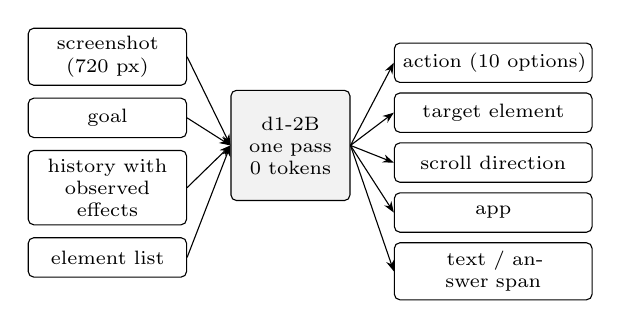
\begin{tikzpicture}[
  font=\scriptsize,
  box/.style={draw, rounded corners=2pt, align=center, inner sep=3pt, minimum height=0.5cm},
  arr/.style={-{Stealth[length=4pt]}, thin}]
  \node[box, text width=1.8cm] (s) {screenshot\\(720 px)};
  \node[box, text width=1.8cm, below=0.15cm of s] (g) {goal};
  \node[box, text width=1.8cm, below=0.15cm of g] (h) {history with\\observed effects};
  \node[box, text width=1.8cm, below=0.15cm of h] (e) {element list};
  \node[box, text width=1.3cm, right=0.55cm of g, yshift=-0.35cm, minimum height=1.4cm, fill=gray!10] (m) {d1-2B\\one pass\\0 tokens};
  \node[box, text width=2.3cm, right=0.55cm of m, yshift=1.05cm] (a) {action (10 options)};
  \node[box, text width=2.3cm, below=0.12cm of a] (t) {target element};
  \node[box, text width=2.3cm, below=0.12cm of t] (d) {scroll direction};
  \node[box, text width=2.3cm, below=0.12cm of d] (p) {app};
  \node[box, text width=2.3cm, below=0.12cm of p] (x) {text / answer span};
  \foreach \n in {s,g,h,e} \draw[arr] (\n.east) -- (m.west);
  \foreach \n in {a,t,d,p,x} \draw[arr] (m.east) -- (\n.west);
\end{tikzpicture}
\caption{The decision contract. One forward pass answers five typed questions; the harness
maps the answers to one AndroidWorld action.}
\label{fig:contract}
\end{figure}

\cref{fig:contract} shows the contract.

\textbf{State.} The input at each step is the screenshot plus a text state. The text holds the
goal, a progress line, the current app, and the previous actions, each with the effect the
harness observed after it (``screen changed'' or ``no change''). It ends with the element list
rendered from the accessibility tree. One function renders this state for training, evaluation
and serving, so the three cannot drift apart.

\textbf{Questions.} Each output is a typed choice: the action, from \{click, type, long press,
scroll, wait, back, home, open app, done, answer\}; the target element; the scroll direction;
and the app. Typed text and answers are \emph{pointer reads}, that is, spans copied from the
text state. In d1, span questions read positions of the text input only. The model therefore
cannot produce text that appears only in the pixels (\cref{sec:failures}).

\textbf{Harness.} The harness follows AndroidWorld's official protocol: seeded task instances,
partial credit, termination decided by the agent, and no oracle stop. Every episode header
records the agent policy that produced it.

%% ------------------------------------------------------------------
\section{Training}

\textbf{Schedule.} We fine-tune every parameter of d1-2B except the tied embedding and output
head, which stay frozen. The vision encoder is trained too: all 132 vision tensors differ
from the base checkpoint. Training is one epoch of 2{,}482 steps with 16 rows per step and a
learning rate of $10^{-5}$.

\textbf{Data.} The main set has 37{,}977 rows from AndroidControl's train split. They are
rebuilt from the original files, restricted to task kinds similar to AndroidWorld's, and
exclude every test episode. We augment them in five ways:
\begin{itemize}
  \item history lines labelled with the observed effect of each action;
  \item ``no change'' rows, which teach the model not to repeat an action that had no effect;
  \item rows that mark actions to avoid;
  \item the AndroidControl-Low step instruction, shown on a fixed half of the rows;
  \item episodes that end in an answer.
\end{itemize}

\textbf{Disclosure.} A further 1{,}736 rows map goal text from AndroidWorld's own task
generator to the app to open. They cover 97 of the 116 evaluated templates; 19 templates are
held out. No AndroidWorld rollout, screen or checker is used. The rows still expose the model
to AndroidWorld's goal phrasing and app names for most tasks. We do not report a split of
success between covered and held-out templates.

%% ------------------------------------------------------------------
\section{Experiments}

\subsection{Setup and Metrics}

\textbf{AndroidControl.} We use the 8{,}444-step test split (1{,}543 episodes) and InfiGUI's
scorer without changes. \emph{Type} is action-type accuracy. \emph{Grounding} is the share of
click and long-press steps, among those with the right type, whose point lies in the target
element. \emph{SR} is the share of steps where the whole action is right. We also report the
share of episodes in which every step is right. AndroidControl-Low shows the step instruction;
AndroidControl-High shows only the goal. Both feed the demonstrator's history at each step.

\textbf{AndroidWorld.} We run 116 tasks with seed 30, one attempt per task (pass@1), and the
official checker. SR is the sum of task scores over scored tasks, so a partial credit counts as
half. Decoding is argmax, but the environment is not deterministic: in an earlier check,
6 of 20 same-host replays diverged.

\subsection{AndroidControl}

\cref{tab:ac} gives AndroidControl results in the format used by recent papers. The other rows
are copied from MobileRL's Table~2 \cite{mobilerl2025}. Those models use other scorers, other
action spaces and other history handling: MobileRL, for example, keeps the agent's own history
in AndroidControl-High and replaces wrong actions. The rows are therefore not strictly
comparable with ours. On Low, our SR (89.3) is 1.5--6.6 points below every listed row. On High
the gap is larger: 9--16 points on Type and 10--16 points on SR. High grounding (78.4) is
between the MobileRL rows (71.5--78.1) and the UI-TARS and UI-Genie rows (80.5--86.3). Our
model has 2B parameters and generates no tokens; the listed models have 7B--72B and generate
text. Fine-tuning moved High SR from 40.2 (the same model and questions, not fine-tuned) to 61.7,
and whole-episode accuracy from 9.4\% to 22.3\%.

\begin{table*}[t]
\centering
\caption{AndroidControl test set (8{,}444 steps). Type = action-type accuracy; Grounding =
target accuracy on click and long-press steps with the right type; SR = step success rate. Rows
above the line are copied from MobileRL, Table~2 \cite{mobilerl2025} (scorers and protocols
differ; not strictly comparable). Our rows use InfiGUI's scorer.}
\label{tab:ac}
\small
\setlength{\tabcolsep}{4pt}
\begin{tabular}{@{}l c c ccc ccc@{}}
\toprule
& & & \multicolumn{3}{c}{AndroidControl-Low} & \multicolumn{3}{c}{AndroidControl-High} \\
\cmidrule(lr){4-6}\cmidrule(l){7-9}
Model & Params & Tokens & Type & Grounding & SR & Type & Grounding & SR \\
\midrule
UI-TARS-7B            & 7B  & yes & 98.0 & 89.3 & 90.8 & 83.7 & 80.5 & 72.5 \\
UI-TARS-72B           & 72B & yes & 98.1 & 90.8 & 91.3 & 85.2 & 81.5 & 74.7 \\
UI-Genie-7B           & 7B  & yes & 98.1 & 89.3 & 94.3 & 83.5 & 82.9 & 74.5 \\
UI-Genie-72B          & 72B & yes & 98.3 & 95.4 & 94.8 & 84.9 & 86.3 & 77.0 \\
MobileRL-7B w/o RL    & 7B  & yes & 96.7 & 93.7 & 91.9 & 87.0 & 73.6 & 72.8 \\
MobileRL-7B w/ RL     & 7B  & yes & 96.9 & 92.4 & 91.4 & 86.3 & 71.5 & 71.3 \\
MobileRL-9B w/o RL    & 9B  & yes & 98.6 & 95.8 & 95.9 & 89.8 & 78.1 & 77.5 \\
MobileRL-9B w/ RL     & 9B  & yes & 97.9 & 94.6 & 94.3 & 87.0 & 74.5 & 73.9 \\
\midrule
d1-2B, not fine-tuned & 2B & none & \pend & \pend & \pend & 63.6 & 63.1 & 40.2 \\
\textbf{d1-2B decision model (ours)} & 2B & none & \textbf{96.6} & \textbf{90.1} & \textbf{89.3} & \textbf{74.3} & \textbf{78.4} & \textbf{61.7} \\
\bottomrule
\end{tabular}

\vspace{4pt}
\footnotesize
Our counts: Low --- Type 8{,}160/8{,}444, Grounding 4{,}454/4{,}941, SR 7{,}544/8{,}444;
High --- Type 6{,}270/8{,}444, Grounding 3{,}337/4{,}257, SR 5{,}213/8{,}444.
Episodes with every step right: Low 932/1{,}543 (60.4\%), High 344/1{,}543 (22.3\%).
Not fine-tuned d1-2B, High: Type 5{,}371/8{,}444, Grounding 2{,}222/3{,}523, SR 3{,}391/8{,}444; episodes 145/1{,}543 (9.4\%).
\end{table*}

\subsection{Per-Step Accuracy Is Not Task Success}
\label{sec:perstep}

The AndroidControl-High scorer gives the demonstrator's history and screen at every step and
never checks the goal, so errors cannot compound. Whole-episode accuracy shows the compounding
that the per-step rate hides (\cref{tab:eplen}): 59\% of one-step episodes are fully right, but
only 5\% of episodes with ten or more steps.

\begin{table}[t]
\centering
\caption{AndroidControl-High: episodes with every step right, by episode length.}
\label{tab:eplen}
\footnotesize
\setlength{\tabcolsep}{2.4pt}
\begin{tabular}{@{}l rrrrr rrrrr@{}}
\toprule
Steps & 1 & 2 & 3 & 4 & 5 & 6 & 7 & 8 & 9 & $\geq$10 \\
\midrule
Right & 69 & 37 & 70 & 60 & 49 & 19 & 18 & 11 & 4 & 7 \\
Total & 116 & 122 & 200 & 221 & 256 & 173 & 138 & 102 & 65 & 150 \\
\% & 59 & 30 & 35 & 27 & 19 & 11 & 13 & 11 & 6 & 5 \\
\bottomrule
\end{tabular}
\end{table}

The whole-episode rate on AndroidControl-High (22.3\%) is close to the AndroidWorld rate
(21.7\%), but the two measure different things. AndroidWorld is harder because errors compound,
the agent must stop on its own, and 13 of its 20 apps have no training goals. It is easier
because any path that reaches the goal state is accepted. In our runs the two effects roughly
cancel, which makes the episode-level rate the better offline proxy.

Termination explains a large share of the gap. The AndroidControl test set has \emph{no} step
where ``done'' is correct, yet the model predicts ``done'' on 1{,}171 of 8{,}444 steps. Of these,
460 are on an episode's last real step and 566 are on steps whose correct action is a scroll.
The two groups share 186 steps, so they must not be added.

\subsection{AndroidWorld}

The model scores 25/115 = 21.7\% (24 full successes and two half credits). One task,
OsmAndMarker, failed at environment setup and is excluded; the cause is fixed
(\cref{sec:harness}). For reference, on an earlier harness an agent that declares ``done''
at step 0 scores 7/113 = 6.6\%, because some tasks start already satisfied.

\cref{tab:difficulty} breaks the score down by the upstream difficulty labels (61 easy,
36 medium, 19 hard) and \cref{tab:complexity} by complexity level, defined as in MobileRL
(the ceiling of the task's complexity value). The ``optimal'' column averages the upstream
optimal step count over all scored tasks in a row. On the tasks the model solved, it used
5.5 steps on easy tasks where the optimum for those tasks is 3.2, and 6.7 steps on medium
tasks against 5.0, so its successes are not on the shortest path. Our level counts (45/41/9/21)
differ from those MobileRL shows for the same definition (49/41/11/15, read from its figure).

\begin{table}[t]
\centering
\caption{AndroidWorld by difficulty (pass@1). Steps are averages per task; ``succ.'' and
``fail.'' split them by outcome; ``opt.'' is the upstream optimal step count.}
\label{tab:difficulty}
\small
\setlength{\tabcolsep}{4pt}
\begin{tabular}{@{}l r r r r r r r@{}}
\toprule
Difficulty & $n$ & Score & SR (\%) & Steps & succ. & fail. & opt. \\
\midrule
easy   & 61 & 21.0 & 34.4 & 8.5  & 5.5 & 10.1 & 5.0 \\
medium & 36 & 3.0  & 8.3  & 13.0 & 6.7 & 13.6 & 9.0 \\
hard   & 18 & 1.0  & 5.6  & 19.3 & --  & 19.3 & 18.5 \\
\midrule
all    & 115 & 25.0 & 21.7 & 11.6 & 5.7 & 13.2 & 8.4 \\
\bottomrule
\end{tabular}
\end{table}

\begin{table}[t]
\centering
\caption{AndroidWorld by complexity level (ceiling of task complexity, as in MobileRL).}
\label{tab:complexity}
\small
\begin{tabular}{@{}l c c c c@{}}
\toprule
Level & C1 & C2 & C3 & C4 \\
\midrule
Tasks & 45 & 41 & 9 & 21 \\
Score / scored & 19/45 & 5.5/40 & 0/9 & 0.5/21 \\
SR (\%) & 42.2 & 13.8 & 0.0 & 2.4 \\
\bottomrule
\end{tabular}
\end{table}

\subsection{The Harness and the Environment Move the Score}
\label{sec:harness}

\cref{tab:harness} holds the checkpoint and the seed fixed and changes only the harness and the
emulator. The score rose from 15.5 to 25 out of 115. With paired per-task comparisons, the two
steps gave 5 wins and 0 losses ($p=0.062$, sign test) and 5 wins and 1 loss ($p=0.22$).

\begin{table}[t]
\centering
\caption{Same checkpoint, same seed; only the harness and the environment change.}
\label{tab:harness}
\small
\begin{tabular}{@{}l c L{4.4cm}@{}}
\toprule
Harness & Score & Change (paired result vs.\ the row above) \\
\midrule
A & 15.5/115 & -- \\
B & 20.5/115 & answers now reach the checker (every answer had scored 0); a fresh observation when the accessibility tree lags the pixels (cap 8\,s). 5 wins / 0 losses. \\
C & \textbf{25/115} & fresh wait also on page change (cap 20\,s); a working SIM; Chrome first-run screens cleared before the suite. 5 wins / 1 loss. \\
D & \pend & numeric answer format; Back closes the keyboard after typing; Markor and OsmAnd state repaired. Only the 39 affected tasks are re-run. \\
\bottomrule
\end{tabular}
\end{table}

We found four environment defects by reading traces; each produces failures that look like
model failures.
\begin{itemize}
  \item \textbf{Markor} opened on its first-run screens in 6 of 6 Markor episodes on one emulator.
  \item \textbf{OsmAnd}: a database query run as root on a missing database left an empty,
        root-owned marker database. OsmAnd could not open it, so the OsmAndMarker task failed
        setup in 3 of 4 runs.
  \item \textbf{VLC}: the media library stays at ``Loading'' on every emulator. The log shows the
        library rejecting a folder after the task's own setup clears its media table as root.
        This cause is inferred, not proven. The Browse tab still reaches the files.
  \item \textbf{Accessibility}: running \texttt{uiautomator dump} stops AndroidWorld's
        accessibility forwarder.
\end{itemize}

\subsection{The Model Uses the Image}

On the 827-step validation split we replaced every screenshot with a uniform grey image of the
same size (\cref{tab:grey}). Step accuracy fell from 519 to 337. Most of the loss is in
\emph{which kind} of action to take: action-type accuracy fell by 29 points, and typing and
scrolling nearly disappeared. We read this as the model looking for a keyboard or a long list,
but that is our interpretation, not a measurement. Element accuracy given the right type fell
less; note that it is measured on different subsets in the two conditions.

\begin{table}[t]
\centering
\caption{Validation split (827 steps) with real vs.\ uniform grey screenshots.}
\label{tab:grey}
\small
\begin{tabular}{@{}l c c@{}}
\toprule
 & Real & Grey \\
\midrule
Step accuracy & 519/827 & 337/827 \\
Action-type accuracy & 80.0\% & 50.8\% \\
Element, given right type & 271/414 & 124/207 \\
Type-text steps right & 37/53 & 3/53 \\
Scroll steps right & 40/86 & 7/86 \\
\bottomrule
\end{tabular}
\end{table}

\subsection{Latency}

Over 1{,}335 AndroidWorld steps, one decision takes 135\,ms at the median and 181\,ms at the
95th percentile. This is one forward pass on a shared 24\,GB GPU, served over HTTP. The
environment step takes 1{,}624\,ms at the median, so the device, not the model, dominates the
agent loop.

\subsection{What the 91 Failed Tasks Are Made Of}
\label{sec:failures}

We split the failed tasks into four groups. One LLM agent per group, with no shared context,
found the first wrong step of each task from its trace and screenshots and checked the
upstream success condition. \cref{tab:failures} summarises the result.

\begin{table*}[t]
\centering
\caption{First wrong step in the 91 failed AndroidWorld tasks, by group. Counts are tasks.}
\label{tab:failures}
\small
\begin{tabular}{@{}l L{13.0cm}@{}}
\toprule
Group (tasks) & Main causes \\
\midrule
Information retrieval (21) & answer visible but never given (4); answer format (1); wrong navigation (4); date, time or colour reasoning (4); counting across screens (2); answer not expressible in the contract (6) \\
Easy (27) & long press needed (5); \emph{Verify} tasks already satisfied (3); premature done (4); wrong element (4); target scrolled off screen (3); typing replaces instead of appending (2); clipboard chip not in the element list (2); environment or app knowledge (4) \\
Medium/hard (34) & app procedure (7); values that must be computed, such as dates and end times (6); stops after the first of several items (4); environment (3); form fields not filled (3); duplicates across screens (3); long note content (2); VLC (2); single cases (4) \\
Visual (9) & navigation with no reading needed (2); drawing or maze pages (2); text only in pixels (4); arithmetic (1) \\
\bottomrule
\end{tabular}
\end{table*}

By outcome, 51 of the 91 failures ended with a wrong ``done'' (49 scored zero and 2 received
half credit) and 40 ran out of step budget. From the group reports we estimate that about 36
failures are blocked by our constraints of one model, no planner and AndroidControl-only data.
This is an estimate, not a per-task tally. The blocked abilities are:
\begin{itemize}
  \item arithmetic and date computation;
  \item memory across screens (counting, duplicates, transcription);
  \item text that exists only in pixels;
  \item colour or icon meaning with no training labels;
  \item information the accessibility tree does not carry (for example screen brightness), and
        inputs the data cannot teach (clipboard chips, appending to a field).
\end{itemize}
TypeSafe's own guidance assigns this kind of work to code, not to the model
\cite{typesafelimits2026}.

\subsection{Negative Results}

\cref{tab:negative} lists what did not work. Each row is one run unless stated.

\begin{table}[t]
\centering
\caption{Negative results.}
\label{tab:negative}
\small
\begin{tabular}{@{}L{2.6cm} L{5.0cm}@{}}
\toprule
Attempt & Result \\
\midrule
Threshold on p(done) & harmful at every threshold on an earlier offline split \\
Separate ``task done?'' head & redundant: its label equals ``action = done'' on 137/137 rows \\
Masking an action already marked ``no change'' & 2 wins / 2 losses on AndroidWorld; premature stops rose \\
Weight merge 0.3/0.7 with an earlier model & 6 wins / 9 losses \\
Recovery (``go back'') rows & 300-step pilot: validation step accuracy 65.2\% $\rightarrow$ 57.7\%; back predicted where gold is not back 1.9\% $\rightarrow$ 10.0\% \\
``Already satisfied $\rightarrow$ done'' rows & at 10\% of training, false done 108/690 with the rows vs.\ 67/690 without; a third run without them gave 106/690, so the effect is not attributable \\
Early stopping rule at 10\% of training & invalid: on an earlier run, mid-training metrics did not predict final ones \\
\bottomrule
\end{tabular}
\end{table}

\subsection{Zero-Shot Pattern Probes}

We asked the trained model two extra questions it was never trained on (\cref{tab:probes}).
Re-ranking the top five elements with one yes/no question per candidate made element choice
worse, although the gold element is in the top five on about 90\% of rows. Asking ``did the last
action move toward the goal?'' on the next screen separated good from bad transitions with an
AUROC of 0.76. This rests on only 26 negatives.

\begin{table}[t]
\centering
\caption{Zero-shot probes. Val = validation (827 rows, 430 with a target element); AC =
AndroidControl sample (2{,}012 rows, 1{,}224 with a target).}
\label{tab:probes}
\small
\begin{tabular}{@{}l c c@{}}
\toprule
Probe & Val & AC \\
\midrule
Element by trained choice & 286/430 & 821/1{,}224 \\
Top-5 re-rank by yes/no & 261/430 & 772/1{,}224 \\
Gold element in top 5 & 388/430 & 1{,}084/1{,}224 \\
Progress question, AUROC & 0.68 & 0.76 \\
\quad negatives / positives & 10 / -- & 26 / 1{,}550 \\
\bottomrule
\end{tabular}
\end{table}

%% ------------------------------------------------------------------
\section{Limitations}

\begin{itemize}
  \item \textbf{Power.} One seed and one attempt per task. A difference of about five tasks on
        AndroidWorld is within noise (sign test $p\approx0.2$ at 5 wins / 1 loss).
  \item \textbf{Benchmark-derived data.} The goal-to-app rows use AndroidWorld's goal templates.
  \item \textbf{Pending.} The not-fine-tuned baseline on AndroidControl-Low, the latest harness, and a
        retrained model.
  \item \textbf{No same-harness generative baseline.} We did not run a generative 2B model on our
        harness, so the published numbers in \cref{tab:aw-context,tab:ac} are context, not
        comparisons.
  \item \textbf{Taxonomy rigour.} The failure taxonomy comes from LLM agents reading traces, one
        per group, without a second reader or an agreement measure.
\end{itemize}

%% ------------------------------------------------------------------
\section{Conclusion}

A 2B decision model can operate a phone end to end at 135\,ms per decision. On AndroidControl
its per-step accuracy overstates its task success by about a factor of three; its
episode-level accuracy and its AndroidWorld success are both near 22\%. The gap has three
parts: termination (51 of 91 failures end in a wrong ``done''), harness and environment
defects that are worth as much as model changes, and abilities a single pass should not be
asked to provide (arithmetic, dates, memory and pixel-only text). In line with TypeSafe's
guidance, the next steps keep the model for judgments and move computation into code:
(1) verify progress on the next screen, which already shows signal without training;
(2) train per-candidate re-ranking; (3) answer by map--reduce, with the model judging each row
and code counting, summing and formatting.

{\sloppy
\bibliography{refs}
\bibliographystyle{icml2026}
}

\newpage
\appendix
\onecolumn
\section{Artifacts}

Every number in the paper is recomputed from files in the project repository.
\begin{itemize}
  \item AndroidControl per-step predictions (High and Low):
        \path{benchmarks/results/2026-11-12-v4/actest/perstep-*.jsonl}.
  \item AndroidWorld traces: \path{benchmarks/results/2026-11-12-maskenv/} and
        \path{benchmarks/results/2026-11-12-armsAB/}; tables by difficulty and level:
        \path{benchmarks/aw/aw_report.py}.
  \item Failure analysis: \path{benchmarks/results/2026-11-12-failanalysis/}.
  \item Image ablation and changed weights: \path{benchmarks/results/2026-11-12-imgablate/}.
  \item Pattern probes: \path{benchmarks/results/2026-11-12-patterns/}.
  \item AndroidWorld task metadata: \path{references/raw/androidworld-task_metadata.json}.
\end{itemize}

\end{document}
